\documentclass[11pt]{article}
\usepackage[a4paper,margin=1in]{geometry}
\usepackage{graphicx}
\usepackage{booktabs}
\usepackage{float}
\usepackage{hyperref}
\usepackage{listings}
\usepackage{xcolor}
\usepackage{longtable}

\hypersetup{
  colorlinks=true,
  linkcolor=blue,
  urlcolor=blue
}

\lstdefinestyle{pythonstyle}{
  language=Python,
  basicstyle=\ttfamily\small,
  keywordstyle=\color{blue},
  commentstyle=\color{teal},
  stringstyle=\color{purple},
  showstringspaces=false,
  breaklines=true,
  frame=single
}

\title{ICMA Data Assignment: Multi-Asset Time-Series Analysis}
\author{}
\date{\today}

\begin{document}
\maketitle
\tableofcontents
\newpage

\section{Executive Summary}
This report analyses the dataset \texttt{input/ICMA Data Assignment\_data set\_March 2026.xlsx} over the full available horizon (2018-04-18 to 2023-04-17). The analysis is structured around the following topics:
\begin{enumerate}
  \item \textbf{Dataset overview} --- description of each time series and its behaviour over the sample period.
  \item \textbf{Cross-asset correlations} --- strongest positive and negative relationships and their economic interpretation.
  \item \textbf{Correlation regime changes} --- instances where established correlations break down, and why.
  \item \textbf{Drivers of CDX IG spread movements} --- relative importance of equity vs.\ rates, and how this varies over time.
  \item \textbf{Counterintuitive patterns} --- relationships that appear to contradict standard risk premia logic.
  \item \textbf{Fair value modeling} --- candidate models for CDX IG fair value and out-of-sample validation.
\end{enumerate}
All analyses are implemented in Python; code and generated outputs are shipped alongside this report.

\section{Methodology}
\begin{itemize}
  \item \textbf{Data handling:} Excel data loaded into a pandas DataFrame, sorted by \texttt{Date}.
  \item \textbf{Transformations:} Most cross-asset relationships are computed on daily changes (\(\Delta x_t = x_t - x_{t-1}\)) to reduce spurious level correlations.
  \item \textbf{Correlations:} Static full-sample correlation matrix and rolling 60-day correlations to detect regime shifts and correlation breakdowns.
  \item \textbf{Impact test for CDX IG:} OLS on standardized daily changes:
  \[
  \Delta CDXIG_t = \alpha + \beta_1 \Delta S\&P_t + \beta_2 \Delta UST10_t + \beta_3 \Delta VIX_t + \beta_4 \Delta CDXHY_t + \epsilon_t.
  \]
  \item \textbf{Fair value models:} candidate OLS models are estimated on daily changes and compared out-of-sample:
  \[
  \Delta CDXIG_t = \alpha + \sum_i \gamma_i \Delta X_{i,t} + u_t.
  \]
  Predicted changes are then integrated into a model-implied fair-value level path.
\end{itemize}

\section{Dataset Overview}

The dataset covers daily observations from April 2018 to April 2023, a period
that spans the late-cycle expansion of 2018--2019, the COVID-19 pandemic shock
of early 2020, the subsequent monetary and fiscal policy response, the
post-pandemic inflation surge, and the aggressive central-bank tightening
campaigns of 2022--2023. Below we describe each series and its behaviour over
the sample.

\subsection*{Equity indices}

\begin{itemize}
  \item \textbf{S\&P 500 (\texttt{S\&P}).}
    The US large-cap equity benchmark gained approximately 53\% over the
    sample, but the path was far from linear. A sharp sell-off in March 2020,
    triggered by global lockdowns, saw the index fall to 2\,237 before
    substantial Fed easing and fiscal stimulus drove a rapid recovery. It
    reached an all-time high near 4\,800 in January 2022, then retreated
    roughly 20\% during the rate-hiking cycle before partially recovering into
    early 2023.

  \item \textbf{EuroStoxx 600 (\texttt{ESTX600}).}
    The broad European equity benchmark rose approximately 22\% over the
    period, following a broadly similar pattern---a crash to 280 in March 2020,
    a strong recovery, and a high near 494 in early 2022. However, its
    performance lagged US equities, reflecting Europe's greater exposure to the
    energy crisis triggered by the Russia--Ukraine conflict and relatively
    slower earnings growth.
\end{itemize}

\subsection*{Foreign exchange}

\begin{itemize}
  \item \textbf{EURUSD spot rate (\texttt{EURUSD}).}
    The euro depreciated approximately 12\% against the dollar over the sample,
    driven by the Fed tightening faster and more aggressively than the ECB,
    compounded by the European energy crisis. The pair briefly broke below
    parity in September 2022, reaching 0.9594---a level not observed since
    2002---before recovering as the ECB accelerated its own hiking cycle.

  \item \textbf{EURUSD 3-month FX basis swap (\texttt{EURUSD3mBS}).}
    This series measures the cost of swapping EUR for USD funding over three
    months, quoted in basis points. On a point-to-point basis it ended close
    to where it started, but exhibited extreme volatility in between. The most
    notable move was a collapse to --81\,bps in March 2020, reflecting acute
    dollar funding stress as global institutions sought USD liquidity.
    The Fed's emergency swap lines quickly normalised the basis. It
    subsequently swung into positive territory, peaking near +65\,bps, as the
    ECB's rate hikes made EUR funding relatively more expensive.
\end{itemize}

\subsection*{Government bond yields and yield curves}

\begin{itemize}
  \item \textbf{10-year US Treasury yield (\texttt{UST10}).}
    The 10-year yield experienced a significant round-trip: it fell to a
    historic low of 0.51\% in August 2020 as the Fed cut rates to zero and
    launched large-scale asset purchases, then rose to 4.24\% in
    October 2022, driven by persistent inflation and aggressive tightening.
    It ended the sample moderately higher than its starting level.

  \item \textbf{10-year Bund yield (\texttt{DEM10}).}
    The German 10-year benchmark fell into deeply negative territory
    (--0.86\%) during 2019--2020, reflecting the ECB's negative-rate policy
    and safe-haven demand during COVID. The yield turned positive in early 2022
    and peaked at 2.75\% as the ECB pivoted to rate hikes, ending the sample
    materially above its starting level.

  \item \textbf{2-year US Treasury yield (\texttt{UST2}).}
    The 2-year yield bottomed at 0.10\% in 2020--2021 when the Fed held rates
    at the zero lower bound, then rose to 5.07\% as the market priced in
    cumulative Fed hikes of over 500\,bps. The short end led the move higher
    because 2-year rates are more tightly anchored to policy-rate expectations,
    ending the sample significantly above its initial level.

  \item \textbf{2-year Schatz yield (\texttt{DEM2}).}
    The German 2-year yield traded as low as --1.01\%, deep in negative
    territory while the ECB deposit rate sat at --0.50\%. When the ECB began
    hiking in July 2022 it climbed rapidly, peaking at 3.33\%---reflecting
    one of the fastest policy pivots in ECB history---and ending the sample
    well above its starting level.

  \item \textbf{2s--10s US Treasury curve (\texttt{USYC}).}
    The 10-year minus 2-year spread steepened to +158\,bps in early 2021 as
    the market anticipated post-COVID reflation while the Fed held the front
    end at zero. It then inverted sharply, reaching --108\,bps, as the
    2-year yield outpaced the 10-year during the hiking cycle---a classic
    recession warning signal.

  \item \textbf{2s--10s German curve (\texttt{DEYC}).}
    The equivalent German spread was persistently steep during the ECB's
    negative-rate era, then flattened and inverted as ECB tightening pulled the
    short end higher faster than the long end. The transition from a positively
    sloped to an inverted curve mirrored the US dynamic with a lag.
\end{itemize}

\subsection*{Overnight rates}

\begin{itemize}
  \item \textbf{SOFR (\texttt{SOFR}).}
    The Secured Overnight Financing Rate, the Fed's preferred short-term
    benchmark, fell to near zero (0.01\%) in March 2020 following emergency
    inter-meeting rate cuts, then rose steadily to 4.80\% by the end of the
    sample, closely tracking the effective federal funds rate through the full
    hiking cycle.

  \item \textbf{Euro short-term rate (\texttt{ESTR}).}
    The ECB's overnight benchmark was pinned around --0.55\% through 2021,
    reflecting the negative deposit facility rate. It began rising in mid-2022
    and ended at 2.90\%, mirroring the ECB's cumulative 350\,bps of
    tightening.
\end{itemize}

\subsection*{Credit default swap indices}

\begin{itemize}
  \item \textbf{CDX IG 5-year (\texttt{CDX IG}).}
    The North American investment-grade CDS index ended the sample modestly
    wider than its starting level. It rose to 152\,bps during the
    March 2020 liquidity crisis as corporate default concerns intensified. The
    Federal Reserve's decision to backstop the corporate bond market via the
    Secondary Market Corporate Credit Facility (SMCCF) rapidly compressed
    spreads back toward pre-crisis levels. A secondary widening occurred in
    mid-2022 amid recession fears, though materially smaller than the COVID
    episode.

  \item \textbf{CDX HY 5-year (\texttt{CDX HY}).}
    The high-yield counterpart widened to 871\,bps in March 2020, nearly
    tripling from pre-crisis levels, as high-yield issuers were seen as most
    vulnerable to a prolonged shutdown. The recovery was swift but HY spreads
    remained wider than their pre-COVID tights throughout the sample, ending
    materially above the starting level.

  \item \textbf{iTraxx Main IG 5-year (\texttt{ITRX IG}).}
    The European investment-grade CDS index mirrored CDX IG's COVID spike
    (peaking at 139\,bps) and subsequent compression, though European spreads
    were additionally affected by the 2022 energy crisis and sovereign-spread
    concerns in peripheral Europe. It ended the sample moderately wider.

  \item \textbf{iTraxx Crossover 5-year (\texttt{ITRX XO}).}
    The European sub-investment-grade/crossover index peaked at 708\,bps in
    March 2020. Crossover spreads remained structurally wider than pre-COVID
    levels throughout the sample, partly reflecting lingering uncertainty
    around European energy security and the corporate impact of higher rates.
\end{itemize}

\subsection*{Commodities}

\begin{itemize}
  \item \textbf{Brent crude oil (\texttt{CO}).}
    Brent crude gained approximately 49\% over the sample but with significant
    intra-period volatility. It fell sharply in early 2020 as lockdowns
    destroyed transport fuel demand, then rose above \$100 in mid-2022
    following Russia's invasion of Ukraine and associated supply disruptions.
    Prices moderated into 2023 as demand concerns from the global slowdown
    partially offset tight supply.
\end{itemize}

\subsection*{Inflation breakevens}

\begin{itemize}
  \item \textbf{US 5-year inflation breakeven (\texttt{US5BEI}).}
    On a point-to-point basis the breakeven ended near its starting level,
    but the intra-sample range was notable: it fell to 0.18\% in March 2020
    as markets priced in a deflationary demand shock, then rose to 3.73\% by
    mid-2022 as realised CPI inflation exceeded 9\%. The magnitude of this
    round-trip was among the largest observed historically, reflecting a rapid
    transition from deflation expectations to sustained above-target inflation.

  \item \textbf{French 5-year inflation breakeven (\texttt{FR5BEI}).}
    This series is excluded from all quantitative analyses due to insufficient
    data coverage (85\% of observations missing). A detailed justification is
    provided in the sensitivity document (Section~2).
\end{itemize}

\subsection*{Volatility}

\begin{itemize}
  \item \textbf{VIX (\texttt{VIX}).}
    The CBOE implied-volatility index ended the sample near its starting
    level, consistent with the VIX's well-known mean-reverting properties. The
    defining event was a rise to 82.7 in March 2020---its
    highest reading since the 2008 financial crisis---as markets experienced
    extreme dislocations. It subsequently mean-reverted, with periodic
    flare-ups during the 2022 sell-off, before settling back near long-run
    averages.
\end{itemize}

\section{Cross-Asset Correlations}
The correlation matrix below is computed on daily changes across the entire sample (April 2018 -- April 2023).

\subsection*{Strong Positive Correlations (daily changes)}
\begin{itemize}
  \item ITRX IG vs ITRX XO: \(+0.9247\)
  \item CDX IG vs CDX HY: \(+0.8240\)
  \item DEM10 vs DEM2: \(+0.8192\)
  \item UST10 vs UST2: \(+0.7525\)
\end{itemize}
Interpretation: these are mostly same-asset-family and same-region risk-factor structures (credit with credit, curve points with curve points).

\subsection*{Strong Negative Correlations (daily changes)}
\begin{itemize}
  \item S\&P vs CDX HY: \(-0.7810\)
  \item S\&P vs VIX: \(-0.7746\)
  \item ESTX600 vs ITRX XO: \(-0.7505\)
  \item S\&P vs CDX IG: \(-0.7104\)
\end{itemize}
Interpretation: classical risk-on/risk-off behavior where equity up-days typically coincide with tighter credit spreads and lower implied volatility.

\begin{figure}[H]
  \centering
  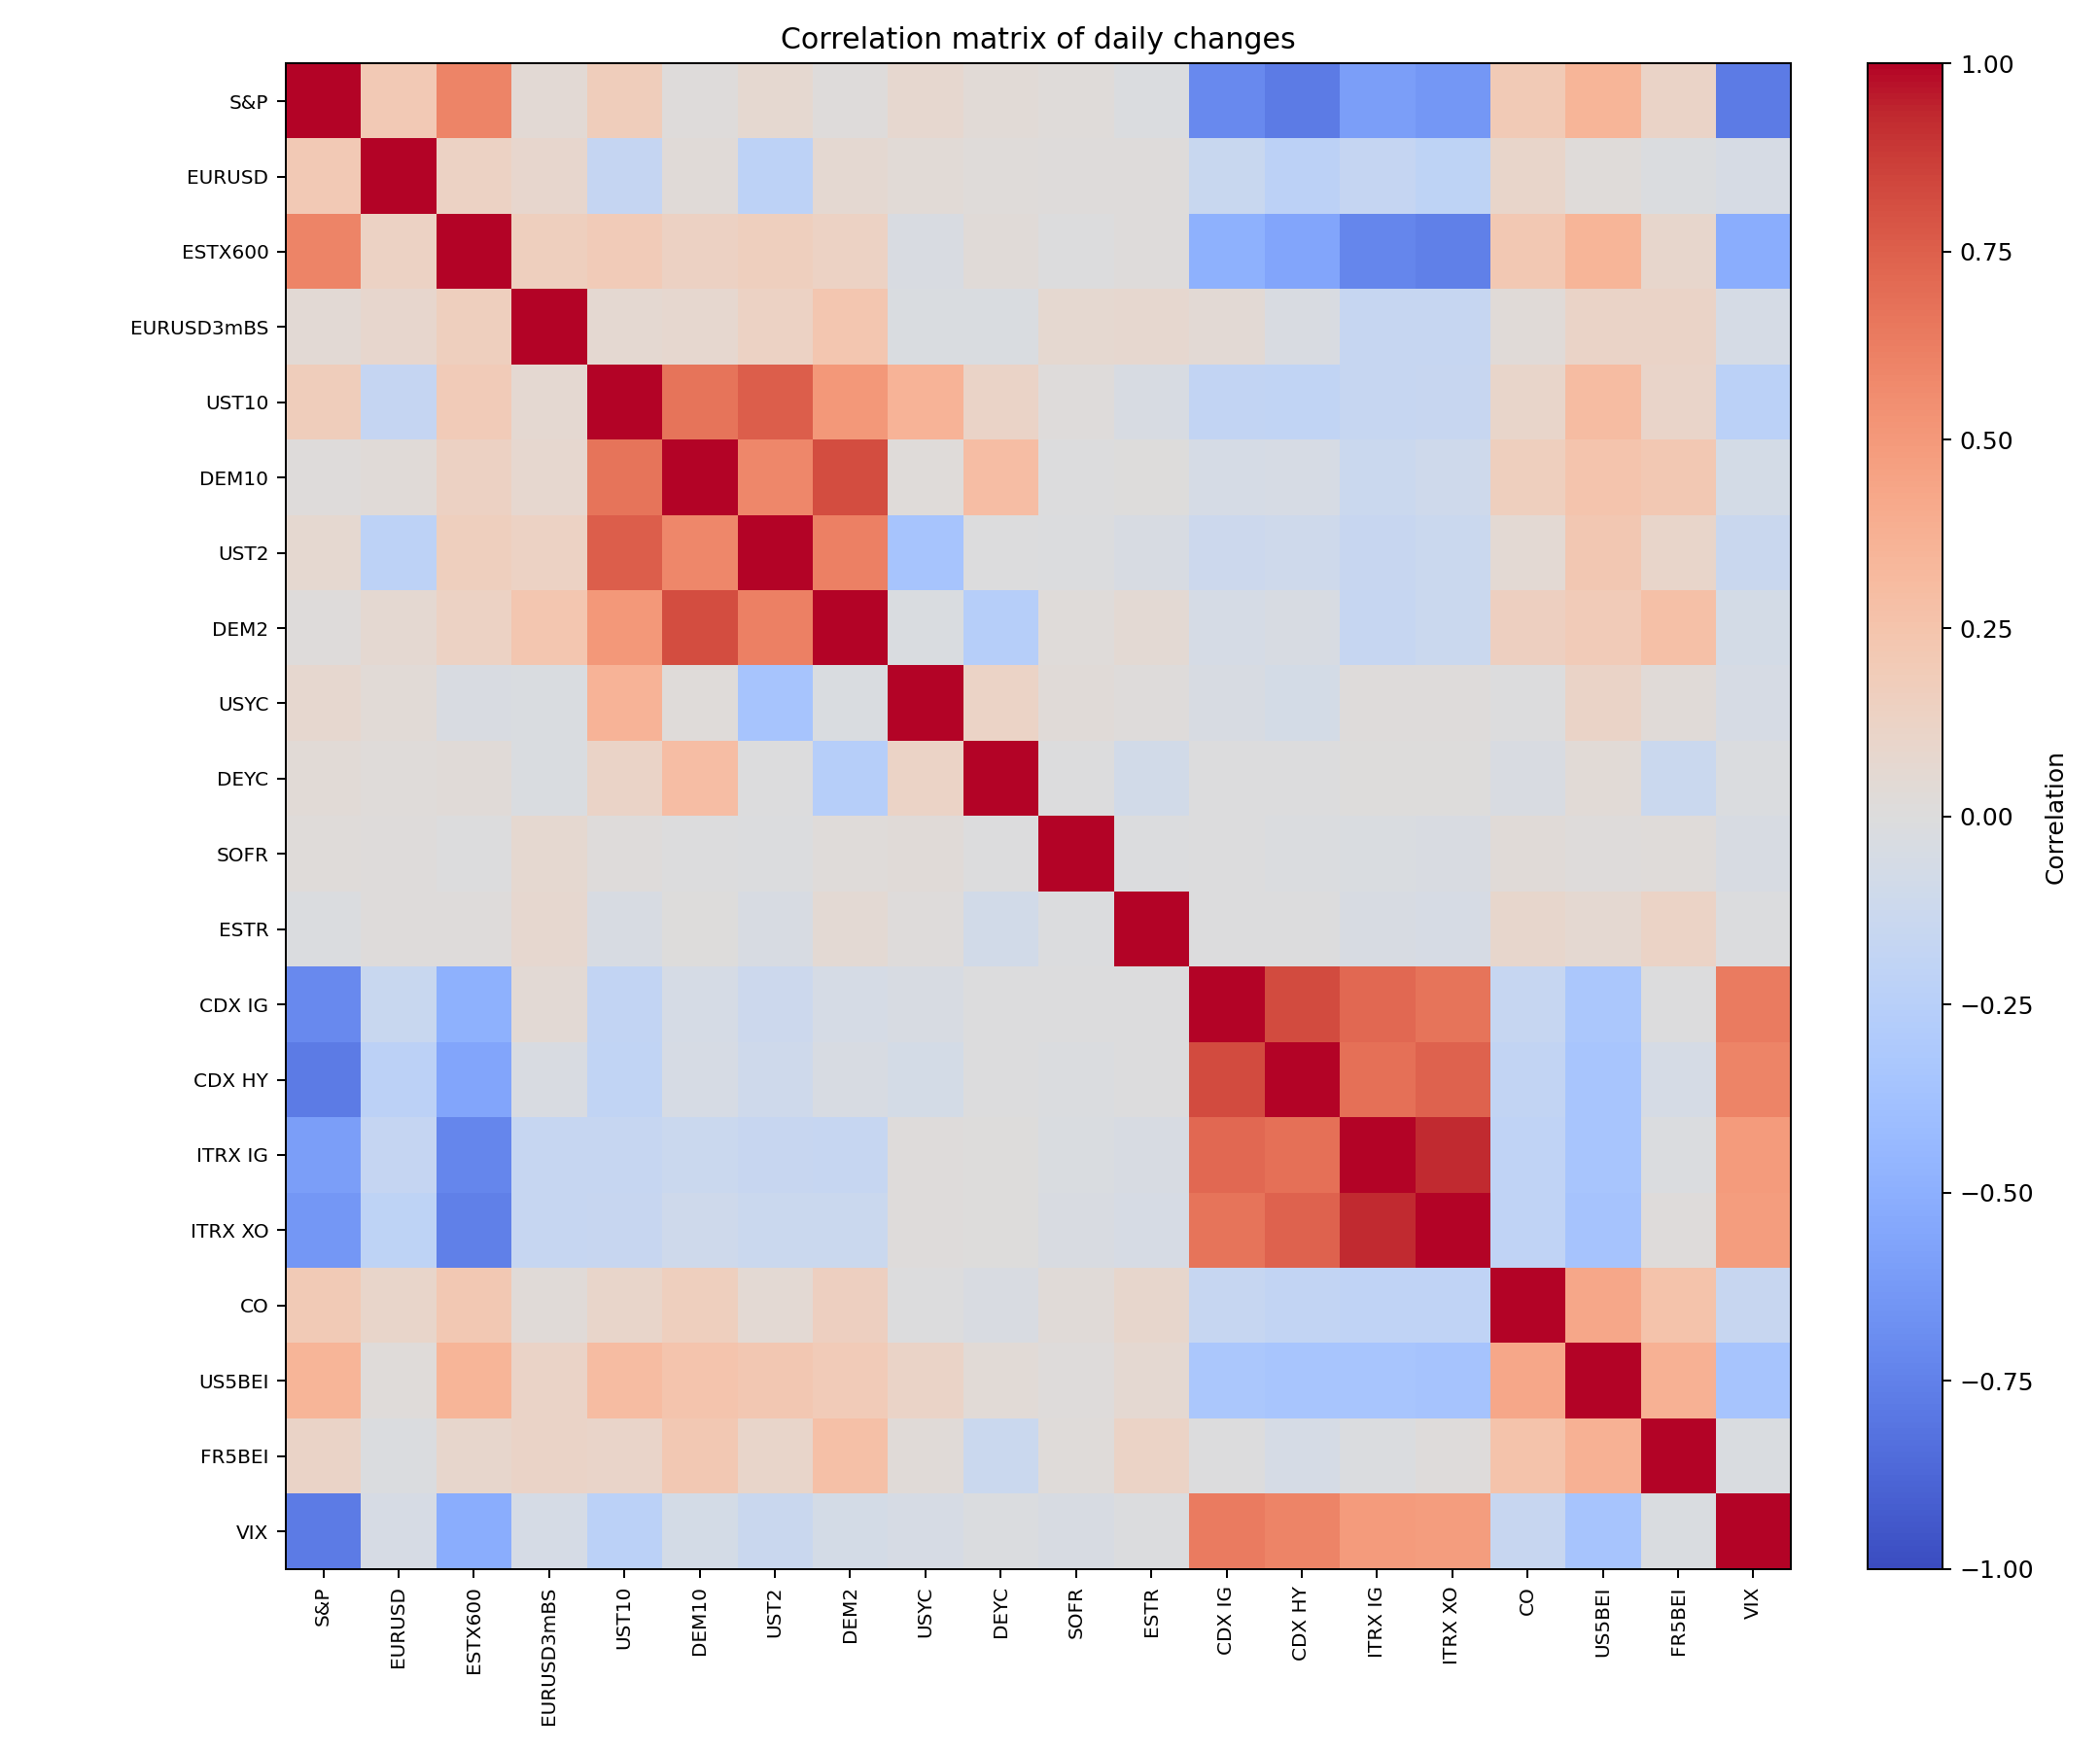
\includegraphics[width=\textwidth]{../../../output/figures/corr_heatmap_changes.png}
  \caption{Correlation matrix of daily changes across all variables.}
\end{figure}

\section{Correlation Regime Changes}
Rolling 60-day correlations show clear regime changes:
\begin{itemize}
  \item S\&P vs UST10 ranges from \(-0.48\) to \(+0.79\), indicating sign flips.
  \item CDX IG vs UST10 ranges from \(-0.82\) to \(+0.48\), another clear breakdown from stable one-sign relationships.
  \item CDX IG vs S\&P remains negative throughout but weakens materially in some windows (from about \(-0.92\) to \(-0.27\)).
\end{itemize}

Economic interpretation:
\begin{itemize}
  \item During acute stress windows, rates and credit can move together as policy expectations and growth fears dominate simultaneously.
  \item In inflation-driven tightening regimes, rates can rise while growth-sensitive assets struggle, changing conventional sign patterns.
  \item Liquidity and technical flows can temporarily dominate macro betas, especially around major event windows.
\end{itemize}

\begin{figure}[H]
  \centering
  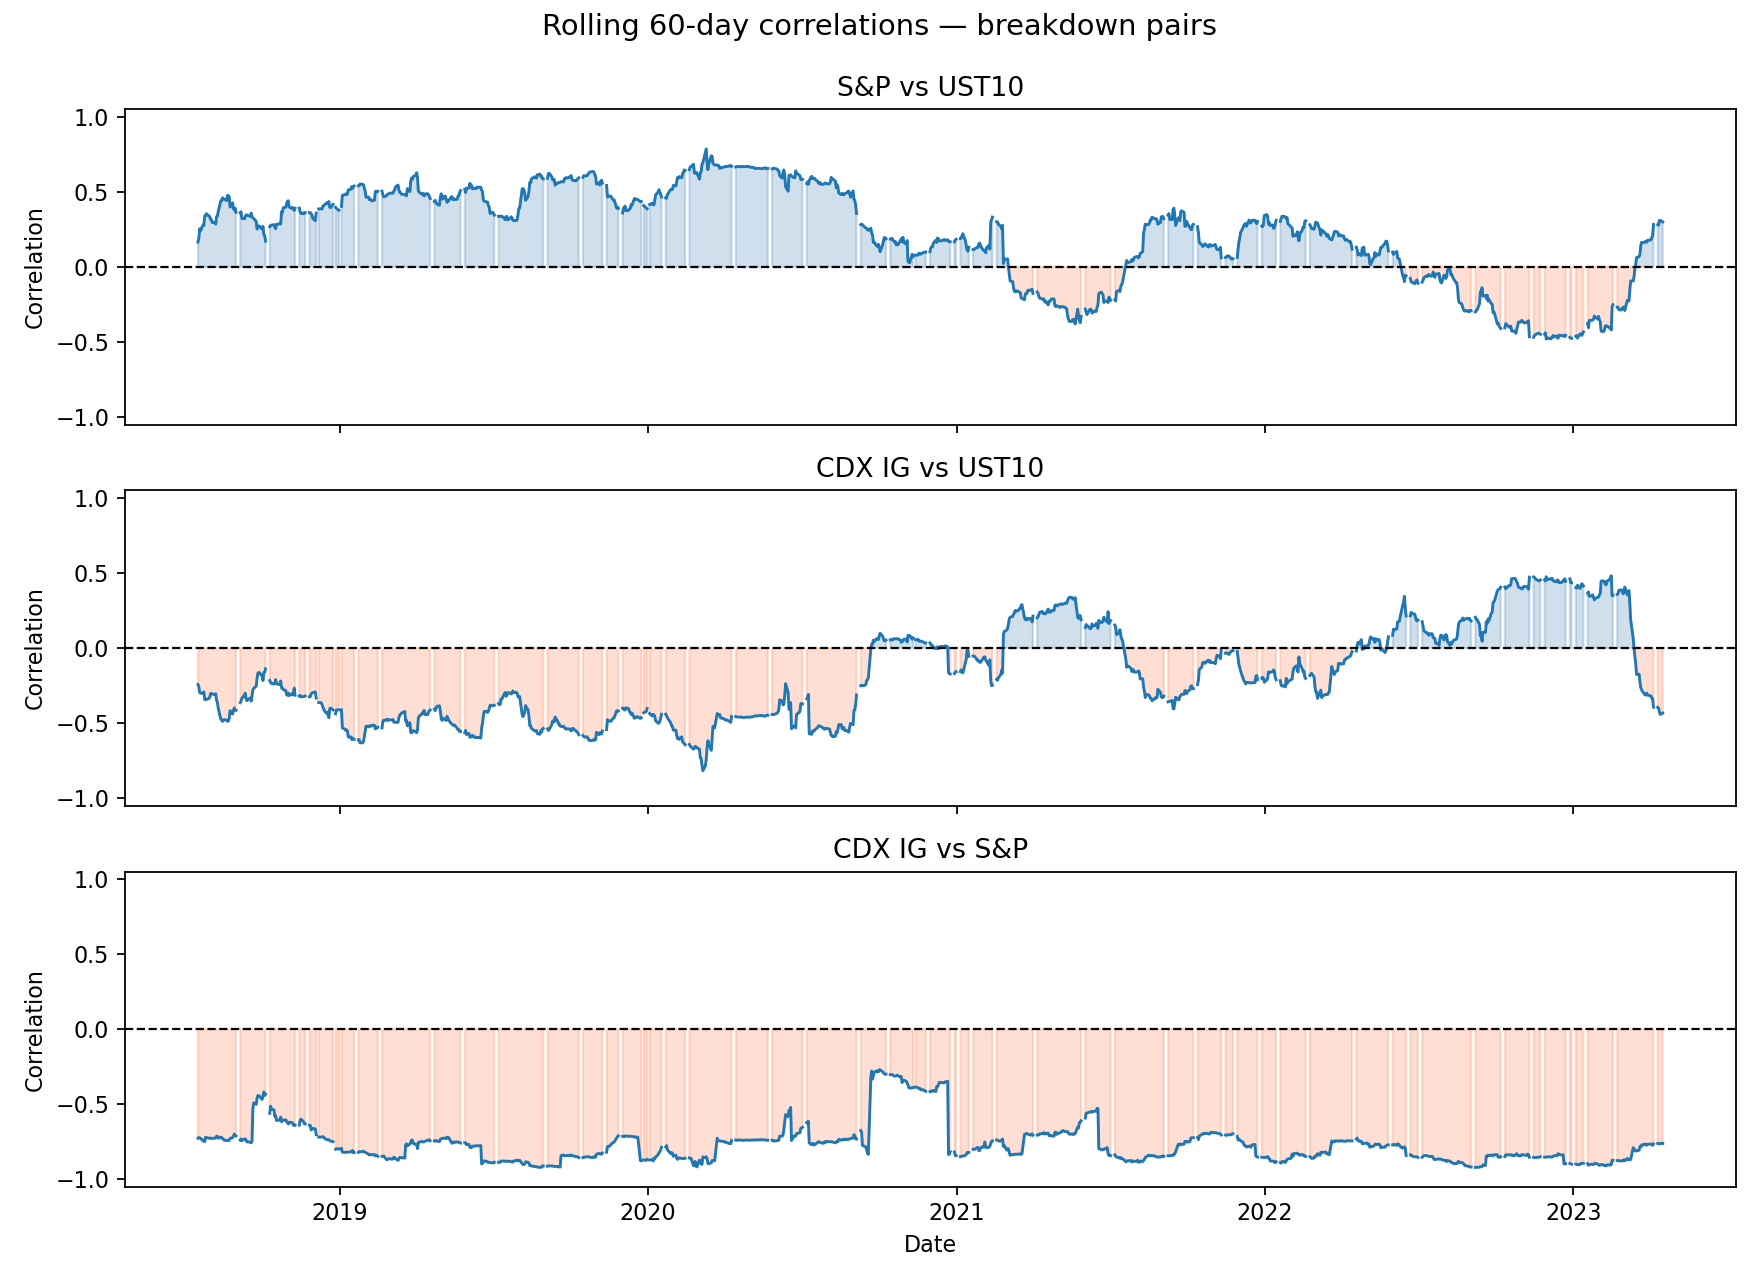
\includegraphics[width=\textwidth]{../../../output/figures/rolling_correlations.png}
  \caption{Rolling 60-day correlations for the three pairs exhibiting sign flips or material breakdowns. Positive regions shaded in blue, negative in red.}
\end{figure}

\section{Drivers of CDX IG Spread Movements}
In standardized multivariate daily-change regressions:
\begin{itemize}
  \item \(\beta_{S\&P} \approx +0.006\)
  \item \(\beta_{UST10} \approx +0.002\)
  \item \(\beta_{VIX} \approx +0.226\)
  \item \(\beta_{CDXHY} \approx +0.694\)
  \item Model \(R^2 \approx 0.711\)
\end{itemize}

Conclusion: S\&P impact is larger than UST10 in this setup, but both are small compared with direct credit and volatility channels (especially CDX HY, then VIX).

Time variation: rolling 60-day pairwise correlations (see \emph{Correlation regime changes}) show substantial shifts in the co-movement of CDX IG with UST10 and with S\&P, including sign changes for the credit--rates pair; these patterns complement the static regression coefficients above.

Further sensitivity checks---including data quality, full OLS diagnostics for all candidate fair-value models, lag and cross-correlation structure, and rolling-window fair value versus the static specification---are provided in the companion document \emph{Sensitivity to Methodology}.

\section{Counterintuitive Patterns}

Several relationships in the dataset deviate from textbook expectations during
specific periods. Below we identify each pattern, the dates at which it
manifests, and the economic rationale.

\subsection*{CDX IG and UST10: positive correlation}

Under normal conditions, investment-grade credit spreads widen when Treasury
yields fall (flight-to-quality), producing a negative correlation. However, the
rolling 60-day correlation turned positive in two distinct episodes:

\begin{itemize}
  \item \textbf{Q1--Q2 2021} (March--July, peak \(+0.34\)). Vaccine
    deployment and large-scale fiscal stimulus supported a broad reflation in
    asset prices. Yields rose on higher inflation expectations, while IG
    spreads widened as the market repriced the term premium and the likelihood
    of an earlier-than-anticipated start to monetary tightening. Both moved
    higher simultaneously, producing a positive correlation.

  \item \textbf{H2 2022 -- Q1 2023} (June 2022--March 2023, peak \(+0.48\)).
    The Federal Reserve was conducting cumulative rate increases of over
    400\,bps during this period, and both yields and spreads were driven
    higher by the same factor: persistently above-target inflation requiring
    sustained monetary tightening. Higher policy rates raised corporate funding
    costs and recession probability simultaneously, causing credit and rates to
    sell off together---a regime in which the traditional negative spread--yield
    relationship breaks down.
\end{itemize}

\subsection*{Crude oil and CDX HY: sign reversal}

Oil and high-yield credit are typically positively correlated through the growth
channel: robust demand supports both oil prices and HY issuers (a significant
share of which, in the US, are energy producers). The rolling correlation was
positive for most of the sample but reversed in early 2022:

\begin{itemize}
  \item \textbf{Pre-2022}: the correlation was negative to near-zero (averaging
    roughly \(-0.20\) to \(-0.40\)), consistent with an environment where oil
    supply shocks and OPEC dynamics dominated---rising oil prices were
    associated with cost-push inflation fears rather than demand strength,
    weighing on HY credit.

  \item \textbf{March--May 2022} (peak \(+0.46\)). Following Russia's invasion
    of Ukraine, oil prices rose above \$100 on supply disruption concerns. HY
    spreads widened concurrently as recession probability increased. As both
    subsequently declined---oil on weakening demand expectations, HY spreads on
    partial relief from peak tightening fears---the correlation turned strongly
    positive. During this period, oil functioned primarily as a geopolitical
    supply-risk indicator rather than a demand proxy, aligning its
    directional moves with those of credit spreads.
\end{itemize}

\subsection*{S\&P 500 and UST10: persistent sign flips}

Equities and Treasury yields can be positively or negatively correlated
depending on whether the dominant macro driver is growth or inflation:

\begin{itemize}
  \item \textbf{2019 -- mid-2020} (peak \(+0.79\)). The correlation was
    strongly positive as both equities and yields were driven by growth
    expectations. In 2019 the Federal Reserve was reducing rates in response
    to slowing growth and trade-policy uncertainty; equities and yields
    declined together. During the COVID-19 sell-off (February--March 2020) and
    the subsequent recovery, both again moved in tandem---lower on the demand
    shock, higher on the monetary and fiscal policy response.

  \item \textbf{Q1--Q2 2021} (trough \(-0.38\)). The correlation turned
    negative as inflation expectations diverged from equity sentiment. Yields
    rose on reflation repricing while equities were volatile on concerns that
    higher rates would compress valuations---an environment in which
    improving macroeconomic data paradoxically weighed on duration-sensitive
    equities through the discount-rate channel.

  \item \textbf{H2 2022 -- Q1 2023} (trough \(-0.48\)). The correlation was
    persistently negative throughout the period of sustained monetary
    tightening. Higher yields reflected restrictive policy, which directly
    impaired equity valuations. Hawkish policy communications pushed yields
    higher and equities lower, while softer inflation data produced the
    opposite effect. This pattern is characteristic of an inflation-dominated
    regime in which the equity--rate relationship inverts relative to
    growth-dominated periods.
\end{itemize}

\section{Fair Value Modeling}

\subsection*{Motivation}

Investment-grade CDS spreads reflect the market's assessment of corporate
default risk and the compensation demanded for bearing that risk. Conceptually,
the main drivers of IG spreads can be grouped into three channels:

\begin{itemize}
  \item \textbf{Risk appetite and equity markets.} Equity indices are a
    real-time proxy for growth expectations and investor risk appetite. When
    equities decline, the implied probability of corporate distress rises, and
    credit spreads widen. The S\&P 500 captures this channel for US-domiciled
    names.

  \item \textbf{Implied volatility.} The VIX measures the cost of hedging
    equity tail risk. Higher implied volatility signals greater uncertainty
    about future cash flows and asset values, which directly increases the
    credit risk premium embedded in IG spreads.

  \item \textbf{Rates and monetary policy.} Treasury yields and the shape of
    the yield curve affect corporate funding costs, discount rates, and the
    macroeconomic outlook. The 10-year yield (UST10) captures the level of
    long-term rates, the 2s--10s curve (USYC) captures term-structure slope
    and recession expectations, and SOFR captures the stance of near-term
    monetary policy. Together, these variables span the rates environment that
    IG issuers face.
\end{itemize}

A model combining these three channels should capture the principal macro forces
acting on CDX IG without including other credit indices (such as CDX HY) as
regressors, which would make the model largely tautological.

\subsection*{Model comparison and best specification}

Several candidate OLS models were estimated on daily changes
(\(\Delta CDXIG\)) and ranked by out-of-sample performance. For each model, a
single set of coefficients is estimated on the first 80\% of the sample
(training set) and held fixed; the remaining 20\% serves as an out-of-sample
test set on which the model is evaluated with no re-estimation. This static
coefficient approach provides a clean assessment of model stability but assumes
that the relationships between CDX IG and its drivers remain constant over
time---an assumption we relax in the sensitivity document, where a
rolling-window alternative is also examined. The best-performing static
specification is:

\[
\Delta CDXIG_t = \alpha + \gamma_1 \Delta VIX_t + \gamma_2 \Delta S\&P_t
  + \gamma_3 \Delta UST10_t + \gamma_4 \Delta USYC_t
  + \gamma_5 \Delta SOFR_t + u_t
\]

Key results:
\begin{itemize}
  \item Out-of-sample \(R^2 \approx 0.698\) and RMSE \(\approx 1.60\) (in
    daily spread-change units).
  \item Predicted daily changes are integrated from the initial observed level
    to reconstruct a model-implied fair-value path for CDX IG.
  \item Residual dislocations (observed minus fair value): the 95th percentile
    absolute residual is approximately 27\,bps, with 60 flagged observations
    exceeding that threshold.
\end{itemize}

The fact that this specification---spanning risk appetite, volatility, and the
rates complex---achieves nearly 70\% out-of-sample explanatory power confirms
that IG credit spreads are primarily a function of broad macro risk factors
rather than idiosyncratic credit events over this sample.

\subsection*{Practical applications}

\begin{itemize}
  \item \textbf{Dislocation screening:} residual z-scores identify periods
    where observed spreads deviate materially from macro-implied fair value,
    which may signal mean-reversion opportunities or structural breaks.
  \item \textbf{Scenario analysis:} the model can be stressed under
    hypothetical rate, equity, or volatility shocks to estimate the expected
    impact on CDX IG spreads.
  \item \textbf{Regime conditioning:} model robustness could be further
    improved by introducing regime indicators (e.g.\ high-volatility vs.\
    low-volatility environments) to allow coefficients to vary across market
    states.
\end{itemize}

Four candidate specifications were tested, each targeting a distinct
transmission channel:

\begin{description}
  \item[RatesVolEquity\_d] \(\Delta VIX\), \(\Delta S\&P\), \(\Delta UST10\),
    \(\Delta USYC\), \(\Delta SOFR\) --- combines equity risk appetite, implied
    volatility, and the US rates complex.
  \item[CrossMarket\_d] \(\Delta ITRX\;IG\), \(\Delta ITRX\;XO\),
    \(\Delta ESTX600\), \(\Delta EURUSD\), \(\Delta DEM10\) --- captures
    European credit and equity cross-market spillovers together with the
    EUR/USD exchange rate and German sovereign yields.
  \item[InflationMacro\_d] \(\Delta CO\), \(\Delta US5BEI\),
    \(\Delta UST2\), \(\Delta DEM2\) --- focuses on inflation expectations
    (via crude oil and the US breakeven rate) and short-end government yields.
    FR5BEI is excluded due to insufficient data coverage (see sensitivity
    document, Section~2).
  \item[FXBasisPolicy\_d] \(\Delta EURUSD\), \(\Delta EURUSD\;3m\;BS\),
    \(\Delta SOFR\), \(\Delta ESTR\), \(\Delta DEYC\) --- emphasises
    cross-currency funding conditions and central-bank policy rates.
\end{description}

\begin{figure}[H]
  \centering
  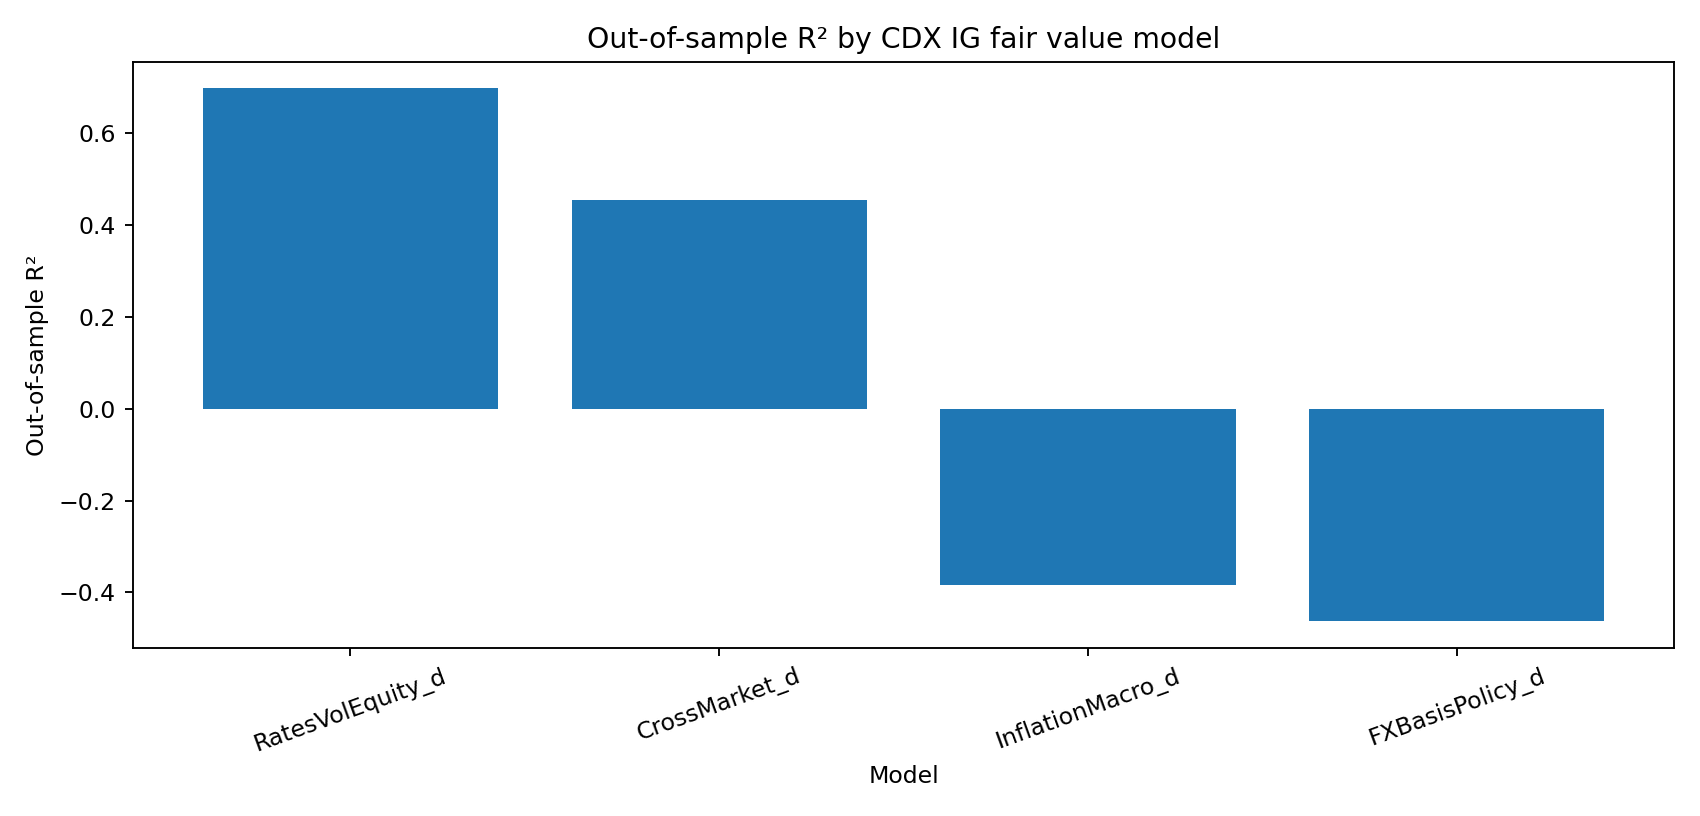
\includegraphics[width=\textwidth]{../../../output/figures/CDX_IG_fair_value_model_comparison.png}
  \caption{Out-of-sample \(R^2\) comparison across alternative CDX IG fair-value models.}
\end{figure}

\begin{figure}[H]
  \centering
  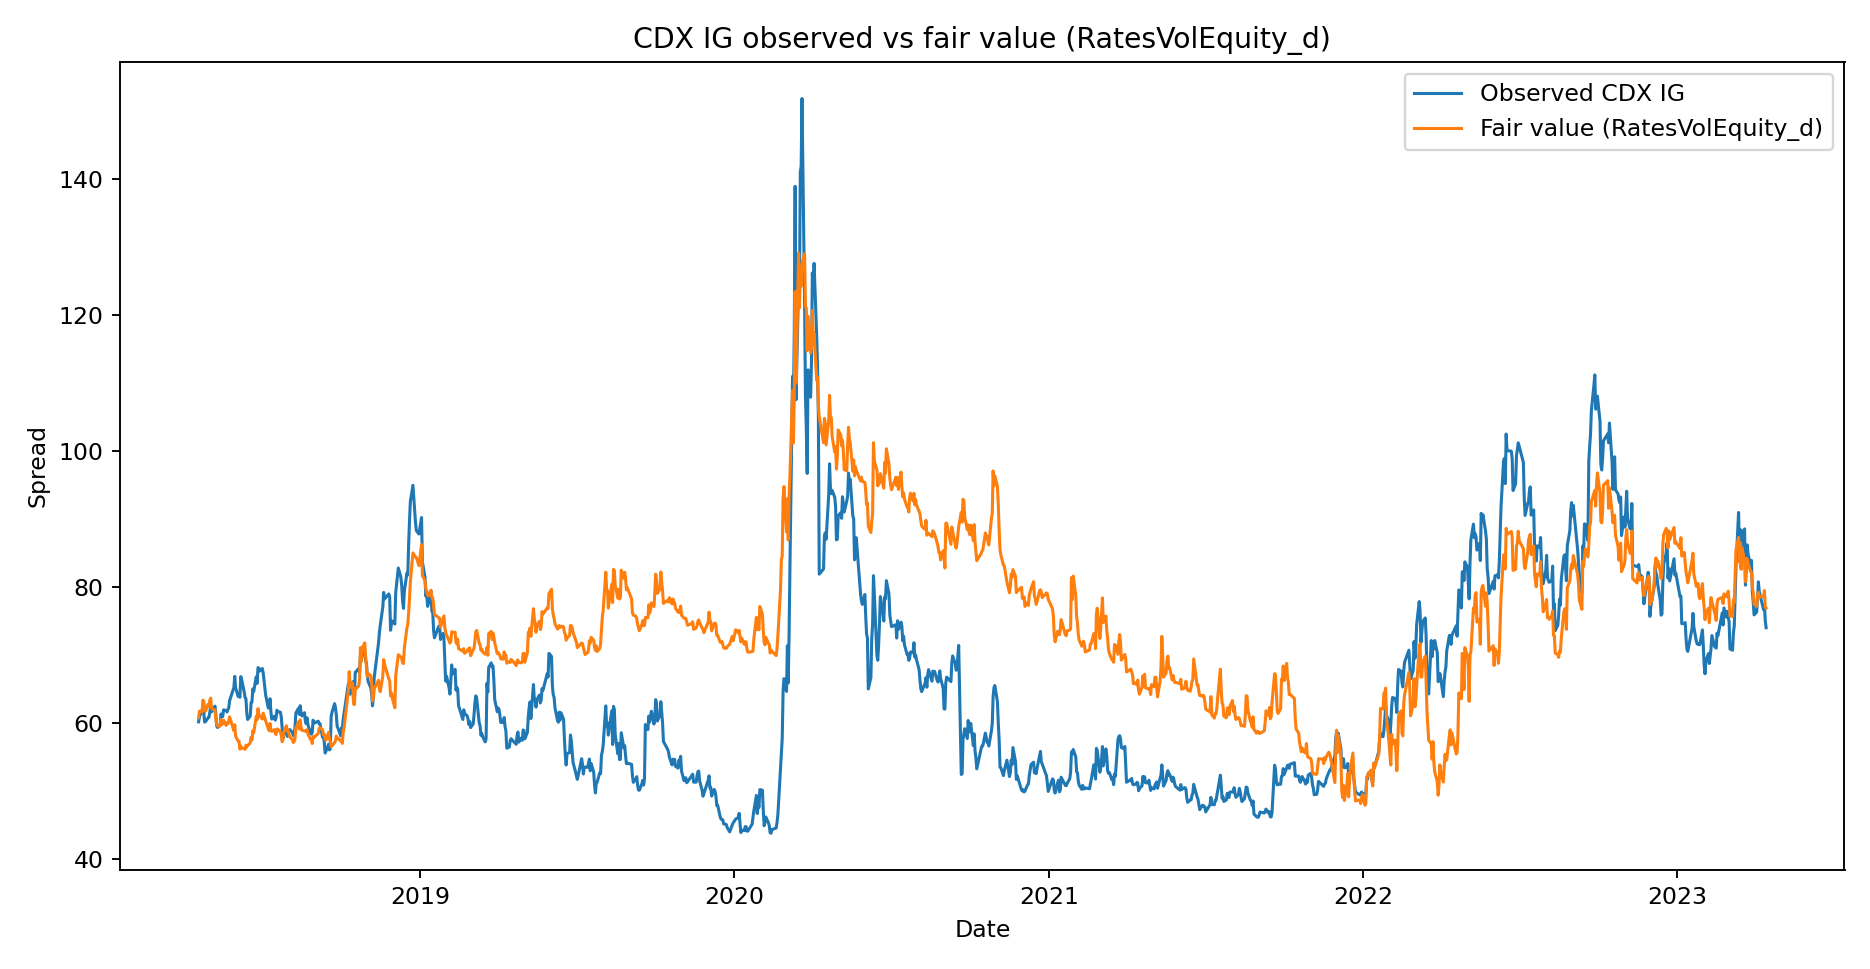
\includegraphics[width=\textwidth]{../../../output/figures/CDX_IG_fair_value_best_model.png}
  \caption{Observed CDX IG vs fair-value level implied by the best change-based model.}
\end{figure}

\section{Reproducibility and Files Generated}
Run:
\begin{lstlisting}[style=pythonstyle]
python3 code/python/analyze_icma_dataset.py
\end{lstlisting}

Main outputs:
\begin{itemize}
  \item \texttt{output/figures/*.png}
  \item \texttt{output/correlation\_changes.csv}
  \item \texttt{output/missing\_value\_statistics.csv}
  \item \texttt{output/CDX\_IG\_fair\_value\_model\_comparison.csv}
  \item \texttt{output/CDX\_IG\_fair\_value\_series.csv}
  \item \texttt{output/CDX\_IG\_rolling\_fair\_value\_series.csv}
  \item \texttt{output/CDX\_IG\_dislocations.csv}
  \item \texttt{output/CDX\_IG\_model\_coefficients\_detail.csv}
  \item \texttt{output/CDX\_IG\_model\_diagnostics\_summary.csv}
\end{itemize}


\appendix
\section{Code Availability}
The analysis code is provided separately in \texttt{code/python/analyze\_icma\_dataset.py}.

\section{Sensitivity to Methodology}
A separate document, \emph{Sensitivity to Methodology}
(\texttt{report/sensitivity\_analysis.pdf}), examines the robustness of the
analytical results presented in this report to alternative methodological
choices. It covers data quality, regression diagnostics across candidate models,
lag structure, and rolling-window fair value relative to the static baseline.


\end{document}
